% arara: pdflatex
% arara: pdflatex

\documentclass{idcannounce}

\textheight 27  cm
\textwidth 17  cm

\usepackage[utf8]{inputenc}
\usepackage[english]{babel}
\usepackage{hyphenat}
\usepackage{newtxmath}
\usepackage[font=scriptsize, labelfont=bf]{caption}
\usepackage{epstopdf}
% \usepackage[pdftex]{graphics}
\usepackage{wrapfig}
\usepackage[acronym]{glossaries}
% wer doch die Computer Modern Roman haben will kann die nächste Zeile aus-auskommentieren
%\renewcommand{\rmdefault}{cmr}
\usepackage{booktabs}
\usepackage{microtype}
\usepackage{picinpar}
\usepackage{tabularx}
\usepackage{pstool}
\usetikzlibrary{positioning}
\usetikzlibrary{patterns}
% use \section* for creating headings

\newacronym{IRS}{IRS}{Intelligent reflecting surface}
\newacronym{CSI}{CSI}{channel state information}
\newacronym{LoS}{LoS}{Line-of-Sight}

\begin{document}
%======================Define Thesis Information Here============================
\def\ThesisType{Research Project}
\def\StudentName{Aakarsh Dhariwal}
\def\Betreuer{Moritz Garkisch}
\def\BetreuerMail{moritz.garkisch@fau.de}
\def\BetreuerRaum{05.040}
\def\Hochschullehrer{Prof. Dr.-Ing. Robert Schober}
\def\ThesisTitel{IRS Codebook Design under Hardware Considerations}
\def\ThesisAusgabe{18.7.22}
\def\ThesisAbgabe{18.10.22}
%================================================================================

%\vspace{-0.2cm}
\heading{\ThesisType} 
\vspace{-1.5cm}
\begin{center}
     \usekomafont{disposition}%
     \large
     \ThesisTitel%
     \\[0.4ex]
     \normalsize for \\ \large\StudentName \\[0.4ex]
%\normalsize for\\
%\large XXXXX
\end{center}

%===============================Put thesis description here======================
%

\begin{wrapfigure}{r}{0.45\textwidth}
    \centering
    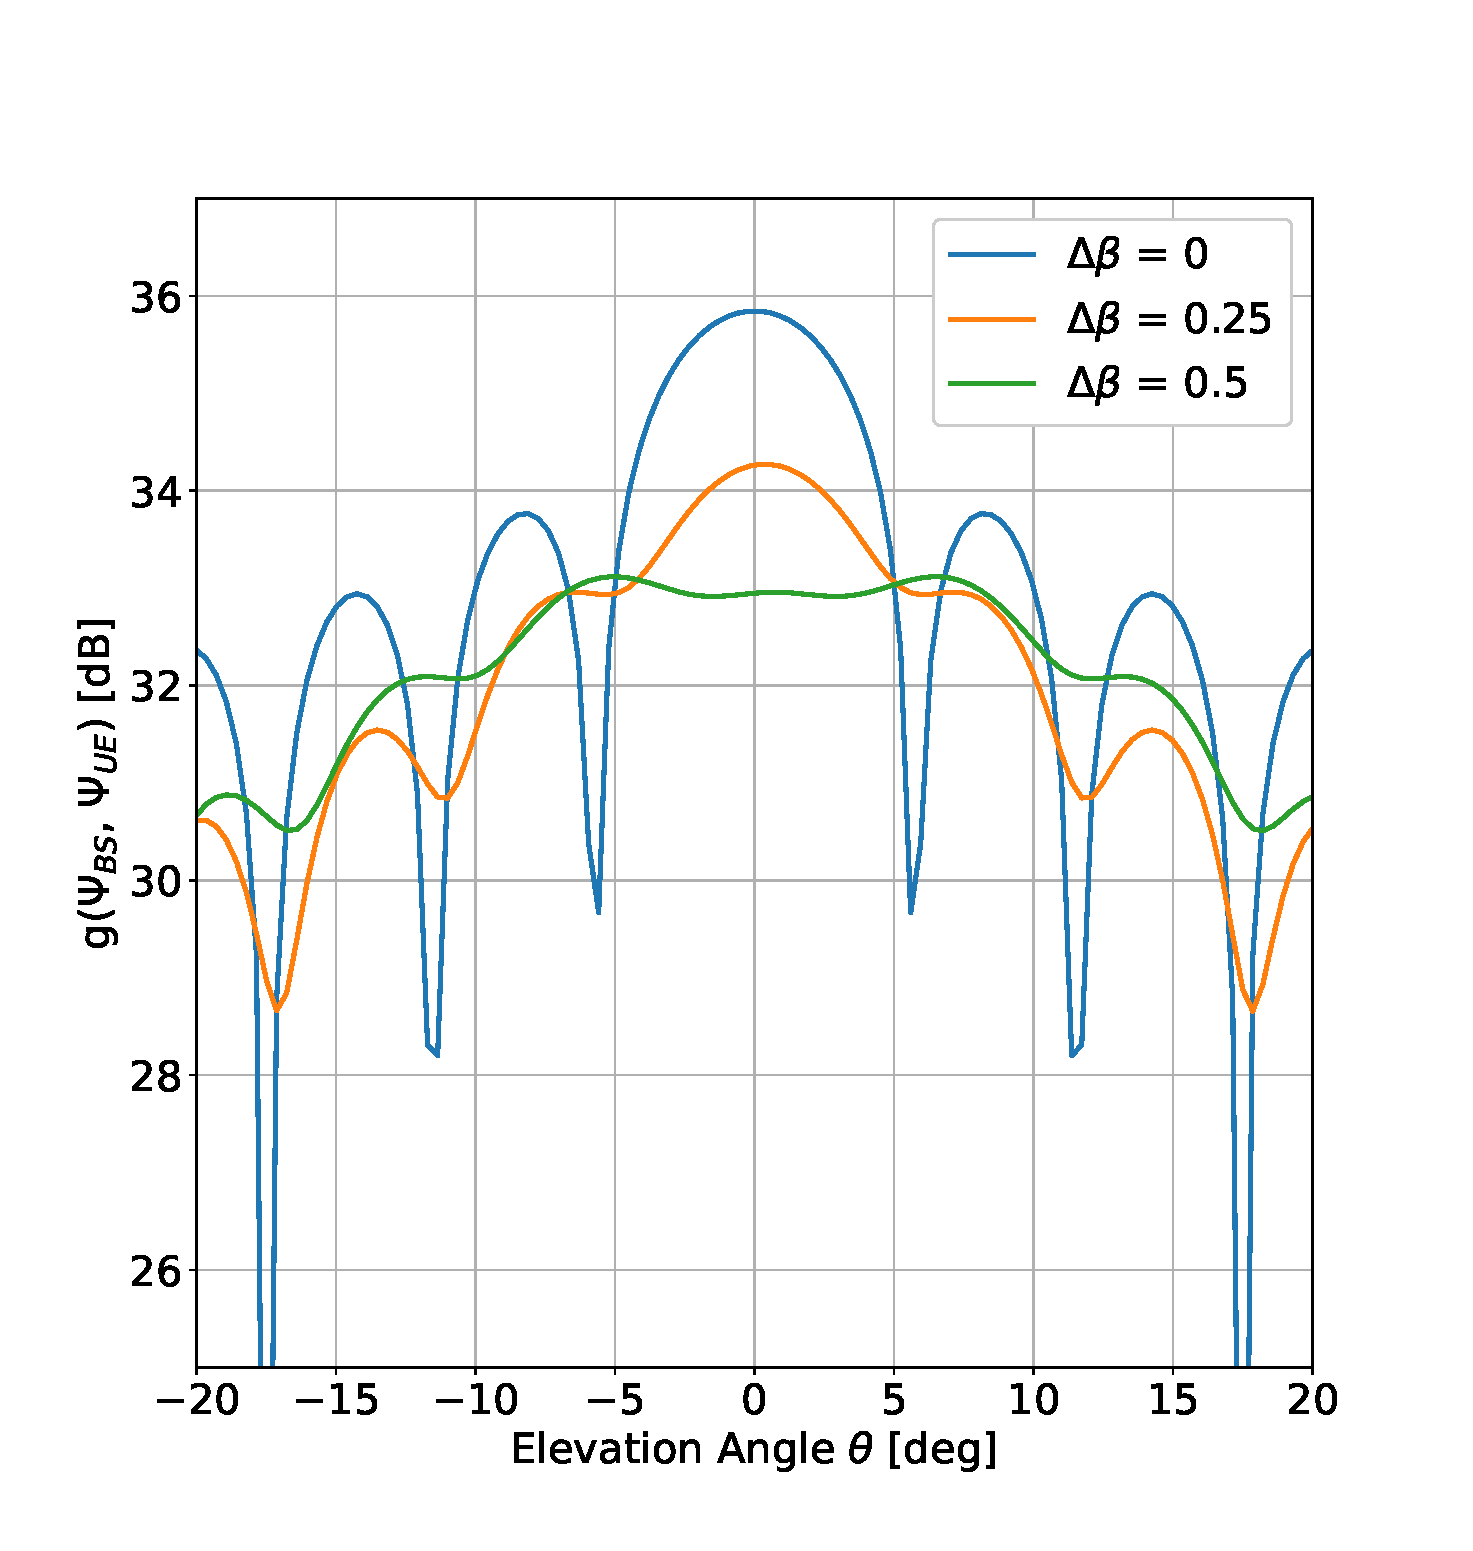
\includegraphics[width=0.45\textwidth]{graphics/var_dbeta.eps}\label{fig:1}
    \caption{Example for \acrshort{IRS} reflection patterns. Here, the parameter $\Delta \beta$ changes the width of the beam.}\label{fig:1}
    \end{wrapfigure}


\glspl{IRS} can provide an additional propagation path in wireless communication systems. This is especially useful for wireless communication systems employing high carrier frequencies if the \gls{LoS} from the transmitter to the receiver suffers from severe attenuation from large objects, such as buildings. \gls{IRS} comprise a large number of unit cells that can apply a phase shift to the reflected electromagnetic waves. The superposition of the reflections from all unit cells leads to reflection behaviors depending on the phases. Early works on \gls{IRS} focused on optimizing the phase shifts for perfect \gls{CSI}. Later, however, the problem of channel acquisition was commonly acknowledged and its necessarily large overhead makes such approaches challenging. To avoid resource-intensive channel estimation, the \gls{IRS} can be configured by selecting predefined codewords from a codebook, which can be done based on measurements of the user's direction. An example for the beam pattern of three different codewords targeting the same direction, but with different beamwidth is shown in Figure \ref{fig:1}. In this project, a codebook that is suitable for the near-field shall be derived. In the practical implementation of \gls{IRS} hardware, the codebooks are limited by the \gls{IRS} technology, e.g., copper patches adjusted by PIN diodes. Therefore, the limitations and inaccuracies of the hardware shall be considered.  \\

The main guidelines for the project are as follows:
\begin{itemize}
\item Literature review on IRS models and codebook designs.
\item Comparison of existing codebooks under hardware impairments and near-field assumption.
\item Design of a robust codebook  suitable for the near-field under hardware impairments.
\end{itemize}
%
%================================================================================
\vfill
\begin{tabularx}{\textwidth}{ll}
     \midrule
     \textsc{Prerequisites}  & Knowledge of digital communication and mathematical optimization.\\
     \textsc{Programming Skills} & Experience in Python or MATLAB.
\end{tabularx}
\begin{tabularx}{\textwidth}{ll}
     \midrule
     \textsc{Supervisors} & \Betreuer, \BetreuerMail, Room \BetreuerRaum \\
			            & Ata Khalili, ata.khalili@fau.de, Room  04.038%,%\\
\end{tabularx}

%\vfill \hspace{0.1\textwidth}
\begin{tabbing}
Start date: \= \ThesisAusgabe\\
End date: \> \ThesisAbgabe
\end{tabbing}
\begin{flushright}
\Hochschullehrer
%\hspace{0.1\textwidth}\null
\end{flushright}

\end{document}
